\documentclass{article}
\usepackage{tikz}
\usepackage{xcolor}

\begin{document}

\begin{figure}[htbp]
    \centering
    % scale 可以調整整張圖的大小
    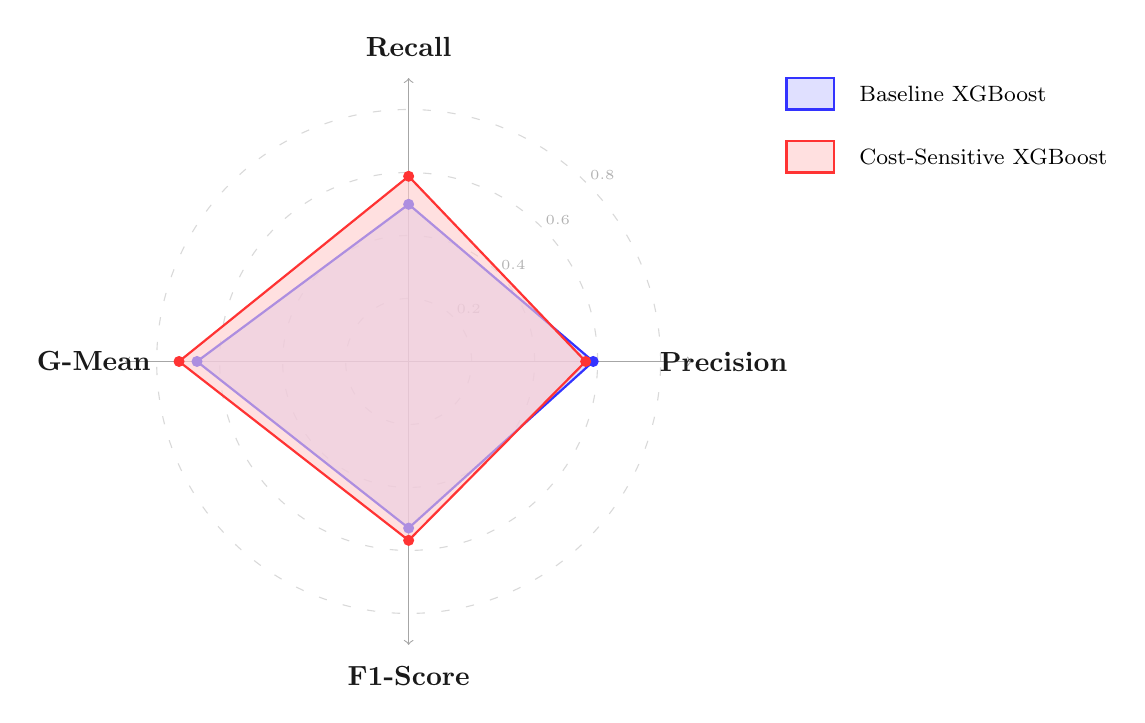
\begin{tikzpicture}[scale=4]
        
        % 1. 畫出背景的蜘蛛網同心圓與刻度 (0.2, 0.4, 0.6, 0.8)
        \foreach \r in {0.2, 0.4, 0.6, 0.8} {
            \draw[gray!30, loosely dashed] (0,0) circle (\r);
            % 在右上角標示數值刻度
            \node[gray!60, anchor=south west, inner sep=1pt, font=\tiny] at (45:\r) {\r};
        }

        % 2. 畫出四條指標的十字軸線
        % 90度: Recall, 0度: Precision, 270度: F1-Score, 180度: G-Mean
        \foreach \angle/\label in {90/Recall, 0/Precision, 270/F1-Score, 180/G-Mean} {
            \draw[gray!70, ->] (0,0) -- (\angle:0.9);
            \node[font=\small, text=black!90, font=\bfseries] at (\angle:1) {\label};
        }

        % 3. 輸入四個資料集(yeast1, 3, 4, 6)的平均實驗數據
        % Baseline XGBoost 平均數據座標 (Recall: 0.499, Precision: 0.586, F1: 0.529, G-Mean: 0.672)
        \coordinate (B_Recall)    at (90:0.499);
        \coordinate (B_Precision) at (0:0.586);
        \coordinate (B_F1)        at (270:0.529);
        \coordinate (B_GMean)     at (180:0.672);

        % CS-XGBoost 平均數據座標 (Recall: 0.588, Precision: 0.562, F1: 0.568, G-Mean: 0.729)
        \coordinate (C_Recall)    at (90:0.588);
        \coordinate (C_Precision) at (0:0.562);
        \coordinate (C_F1)        at (270:0.568);
        \coordinate (C_GMean)     at (180:0.729);

        % 4. 繪製 Baseline XGBoost 藍色多邊形
        \draw[thick, blue!80, fill=blue!20, fill opacity=0.6]
            (B_Recall) -- (B_Precision) -- (B_F1) -- (B_GMean) -- cycle;
            
        % 畫上 Baseline 的資料點
        \foreach \p in {B_Recall, B_Precision, B_F1, B_GMean} {
            \fill[blue!80] (\p) circle (0.5pt);
        }

        % 5. 繪製 Cost-Sensitive XGBoost 紅色多邊形
        \draw[thick, red!80, fill=red!20, fill opacity=0.6]
            (C_Recall) -- (C_Precision) -- (C_F1) -- (C_GMean) -- cycle;
            
        % 畫上 CS-XGBoost 的資料點
        \foreach \p in {C_Recall, C_Precision, C_F1, C_GMean} {
            \fill[red!80] (\p) circle (0.5pt);
        }

        % 6. 圖例 (Legend)
        \begin{scope}[xshift=1.2cm, yshift=0.8cm]
            \draw[thick, blue!80, fill=blue!20, fill opacity=0.6] (0,0) rectangle (0.15, 0.1);
            \node[right, font=\footnotesize] at (0.2, 0.05) {Baseline XGBoost};
            
            \draw[thick, red!80, fill=red!20, fill opacity=0.6] (0,-0.2) rectangle (0.15, -0.1);
            \node[right, font=\footnotesize] at (0.2, -0.15) {Cost-Sensitive XGBoost};
        \end{scope}

    \end{tikzpicture}
    \caption{Radar Chart comparing the average performance of Baseline XGBoost and Cost-Sensitive XGBoost across all datasets.}
    \label{fig:xgboost_average_radar}
\end{figure}

\end{document}